\documentclass[12pt]{beamer}
\newenvironment{ConCodigo}[1]
  {\begin{frame}[fragile,environment=ConCodigo]{#1}}
  {\end{frame}}
\graphicspath{{Imagenes/}{../Imagenes/}}
\usepackage[utf8]{inputenc}
\usepackage[spanish]{babel}
\usepackage{hyperref}
\usepackage{etex}
\reserveinserts{28}
\usepackage{amsmath}
\usepackage{amsthm}
\usepackage{mathtools}
\usepackage{multicol}
\usepackage{multirow}
\usepackage{tabulary}
\usepackage{booktabs}
\usepackage{nccmath}
\usepackage{biblatex}
\usepackage{epstopdf}
\usepackage{graphicx}
%\usepackage{enumitem,xcolor}
\usepackage{siunitx}
\sisetup{scientific-notation=true}
%\usepackage{fontspec}
\usepackage{lmodern}
\usepackage{float}
\usepackage[format=hang, font=footnotesize, labelformat=parens]{caption}
\usepackage[autostyle,spanish=mexican]{csquotes}
\usepackage{standalone}
\usepackage{blkarray}
\usepackage{algorithm}
\usepackage{algorithmic}
\usepackage{tikz}
\usepackage[siunitx]{circuitikz}
\usetikzlibrary{arrows,patterns,shapes}
\usetikzlibrary{decorations.markings}
\usetikzlibrary{arrows}
\usepackage{color}
\usepackage{xcolor}
%\usepackage{beton}
%\usepackage{euler}
%\usepackage[T1]{fontenc}
\usepackage[sfdefault]{roboto}  %% Option 'sfdefault' only if the base font of the document is to be sans serif
\usepackage[T1]{fontenc}
\renewcommand*\familydefault{\sfdefault}
\DeclareGraphicsExtensions{.pdf,.png,.jpg}
\usepackage{hyperref}
\renewcommand {\arraystretch}{1.5}
\newcommand{\python}{\texttt{python}}
\usefonttheme[onlymath]{serif}
\setbeamertemplate{navigation symbols}{}
\usetikzlibrary{patterns}
\usetikzlibrary{decorations.markings}
\tikzstyle{every picture}+=[remember picture,baseline]
%\tikzstyle{every node}+=[inner sep=0pt,anchor=base,
%minimum width=2.2cm,align=center,text depth=.15ex,outer sep=1.5pt]
%\tikzstyle{every path}+=[thick, rounded corners]
\setbeamertemplate{caption}[numbered]
\newcommand{\ptm}{\fontfamily{ptm}\selectfont}
%Se usa la plantilla Warsaw modificada con spruce
\mode<presentation>
{
  \usetheme{Warsaw}
  \setbeamertemplate{headline}{}
  \useoutertheme{default}
  \usecolortheme{seahorse}
  \setbeamercovered{invisible}
}
% \AtBeginSection[]
% {
% \begin{frame}<beamer>{Contenido}
% \normalfont\mdseries
% \tableofcontents[currentsection]
% \end{frame}
%}

\usepackage{listings}
\lstset{ %
language=Python,                % choose the language of the code
basicstyle=\small,       % the size of the fonts that are used for the code
numbers=left,                   % where to put the line-numbers
numberstyle=\footnotesize,      % the size of the fonts that are used for the line-numbers
stepnumber=1,                   % the step between two line-numbers. If it is 1 each line will be numbered
numbersep=5pt,                  % how far the line-numbers are from the code
backgroundcolor=\color{white},  % choose the background color. You must add \usepackage{color}
showspaces=false,               % show spaces adding particular underscores
showstringspaces=false,         % underline spaces within strings
showtabs=false,                 % show tabs within strings adding particular underscores
frame=single,   		% adds a frame around the code
tabsize=4,  		% sets default tabsize to 2 spaces
captionpos=b,   		% sets the caption-position to bottom
breaklines=true,    	% sets automatic line breaking
breakatwhitespace=false,    % sets if automatic breaks should only happen at whitespace
escapeinside={\#}{)}          % if you want to add a comment within your code
}

\usepackage{siunitx}
\usepackage[american,cuteinductors,smartlabels]{circuitikz}
\usetikzlibrary{calc}
\title{Ecuaciones diferenciales ordinarias 3}
\subtitle{Curso de F\'{i}sica Computacional}
\author{M. en C. Gustavo Contreras May\'{e}n}
%\email{curso.fisica.comp@gmail.com}
%\ptsize{10}
\begin{document}
\maketitle
\fontsize{14}{14}\selectfont
\spanishdecimal{.}
\begin{frame}{Contenido}
\tableofcontents[pausesections]
\end{frame}
\section{Ejercicios avanzados.}
\begin{frame}
\frametitle{Ejecicio}
La corriente el\'{e}ctrica de un circuito $RLC$ en serie, satisface la ecuaci\'{o}n\\
\begin{equation} \label{eq:ecuacion1}
	L \frac{di}{dt}+ Ri+ \frac{1}{C} \int_{0}^{t} i(t') dt' +\frac{1}{C}q(0)= E(t), \hspace{0.75cm} t>0 
\end{equation}
cuando el circuito se cierra en el instante $t=0$, se tiene que $i=i(t)$ es la corriente, $R$ es la resistencia, $L,C,E$ vienen dadas por: $L=200H$, $C=0.001F$, $E(t)=1V$ para $t>0$.
\end{frame}
\begin{frame}
\begin{center}
\begin{circuitikz}
\draw
    (0,0)
        to[sV, l=$V_{s}$] ++(0,3)
        to[short] ++(1,0)
        to[cspst, o-o] ++(1,0)
        to[short] ++(1,0)
        to[L, l=$L$] ++(1,0)
        to[short] ++(1,0)
        to[short] ++(0,-1)
        to[C, l=$C$] ++(0,-1)
        to[short] ++(0,-1)
        to[short] ++(-1,0)
        to[R, l=$R$] ++(-1,0) --(0,0);
\end{circuitikz}
\end{center}
Las condiciones iniciales son $q(0)=0$ (carga inicial del condensador), $i(0)=0$. 
\end{frame}
\begin{frame}
Calcular la corriente para $0 \leq t \leq 5$ segundos y el factor de amortiguamiento y la frecuencia de oscilación del circuito $RLC$ para los siguientes valores de R:\\
\begin{enumerate}
	\item $R = 0 \hspace{0.1cm} \Omega$
	\item $R = 50 \hspace{0.1cm} \Omega$
	\item $R = 100 \hspace{0.1cm} \Omega$
	\item $R = 300 \hspace{0.1cm} \Omega$
\end{enumerate}
\end{frame}
\begin{frame}
Si definimos
\begin{equation}\label{eq:ecuacion2}
	q(t) = \int_{0}^{t'} i(t') dt'
\end{equation}
derivando la expresi\'{o}n anterior
\begin{equation}\label{eq:ecuacion3}
	\dfrac{d}{dt}q(t) = i(t), \hspace{1.5cm} q(0)=0
\end{equation}
Sustituimos en la ecuaci\'{o} inicial, para re-escribir
\fontsize{12}{12}\selectfont
\begin{equation}\label{eq:ecuacion4}
	\dfrac{d}{dt}i(t) = -\dfrac{R}{L}i(t) - \dfrac{1}{LC} q(t) + \dfrac{1}{LC}q(0) + \dfrac{E(t)}{L}, i(0)=0 
\end{equation}
La ecuaci\'{o}n (\ref{eq:ecuacion1}) se transform\'{o} en un sistema de dos EDO de primer orden: las ecuaciones (\ref{eq:ecuacion3}) y (\ref{eq:ecuacion4}).
\end{frame}
\begin{frame}
\frametitle{Soluci\'{o}n gr\'{a}fica con $R=0 \Omega$}
\begin{figure}
	\centering
	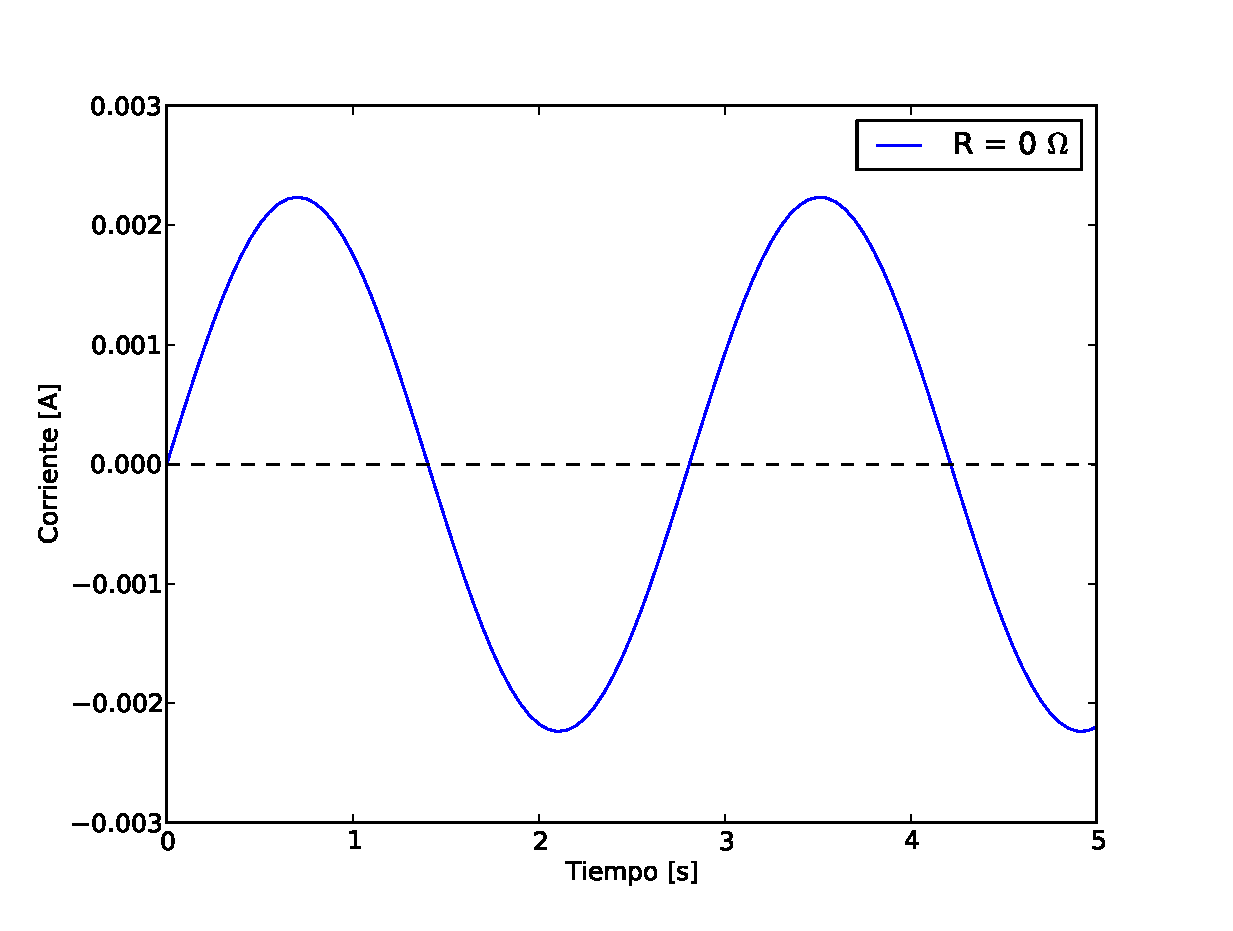
\includegraphics[scale=0.5]{SistemaElecRK4_01.eps} 
\end{figure}
\end{frame}
\begin{frame}
\frametitle{Soluci\'{o}n gr\'{a}fica con $R=50 \Omega$}
\begin{figure}
	\centering
	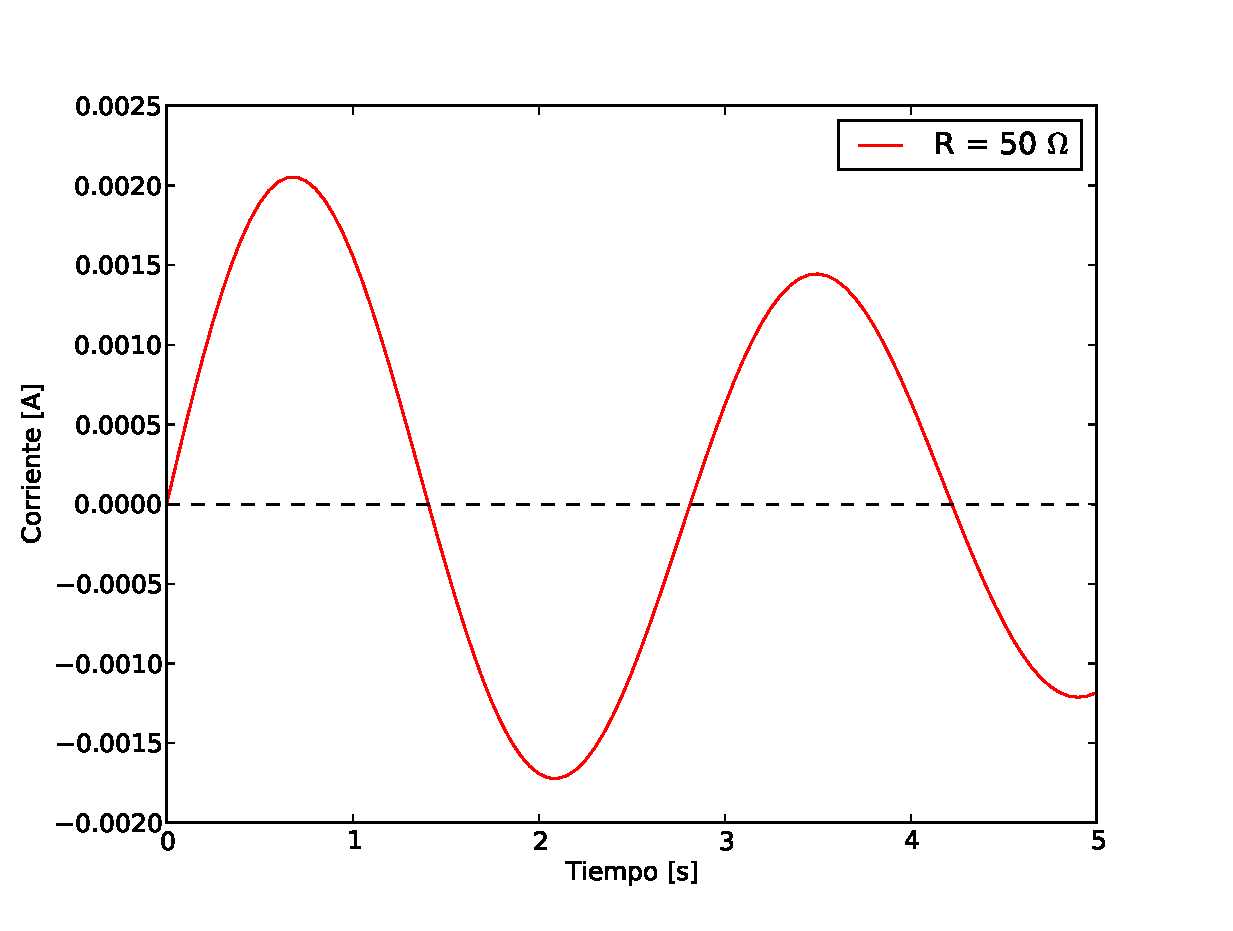
\includegraphics[scale=0.5]{SistemaElecRK4_02.eps} 
\end{figure}
\end{frame}
\begin{frame}
\frametitle{Soluci\'{o}n gr\'{a}fica con $R=100 \Omega$}
\begin{figure}
	\centering
	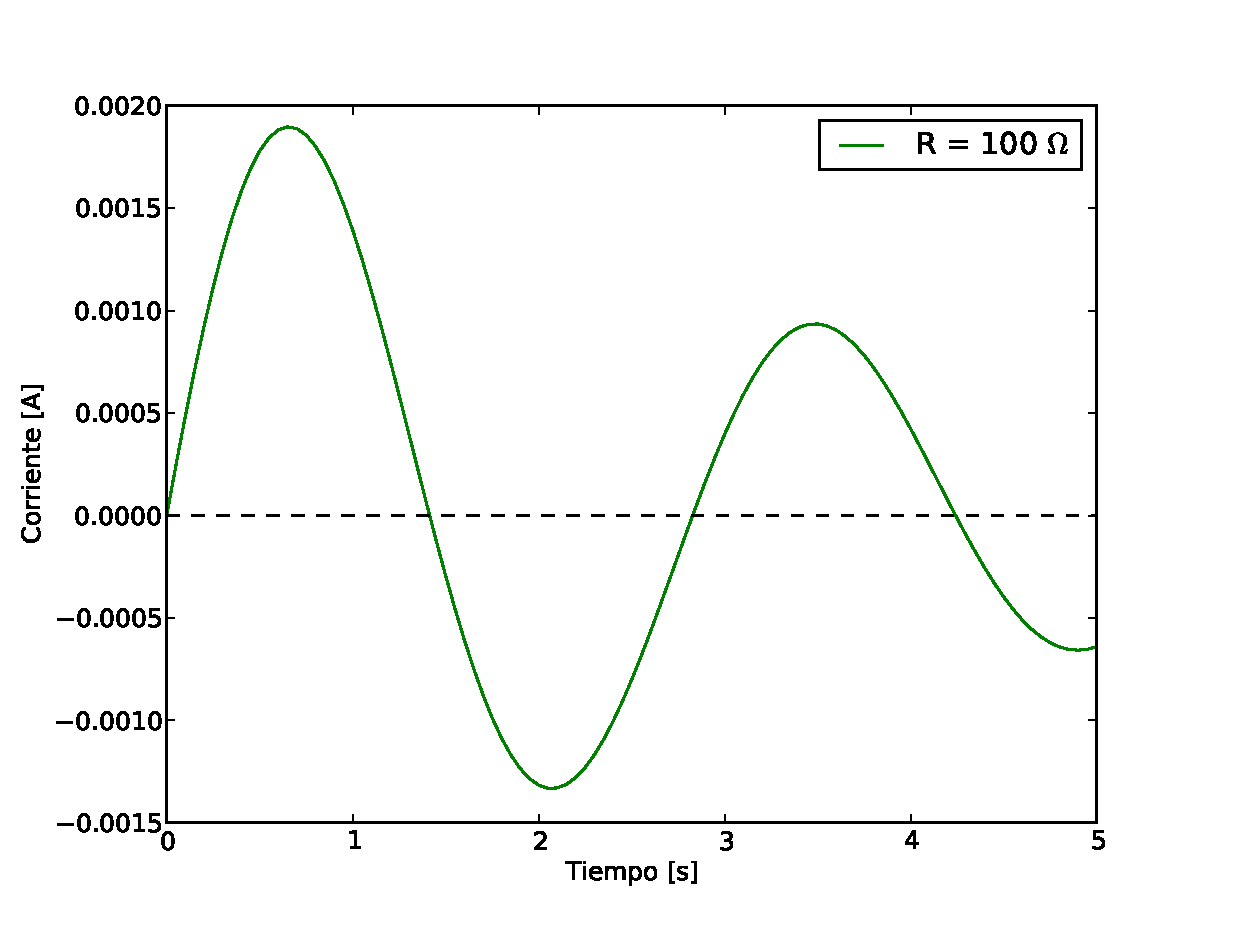
\includegraphics[scale=0.5]{SistemaElecRK4_03.eps} 
\end{figure}
\end{frame}
\begin{frame}
\frametitle{Soluci\'{o}n gr\'{a}fica con $R=300 \Omega$}
\begin{figure}
	\centering
	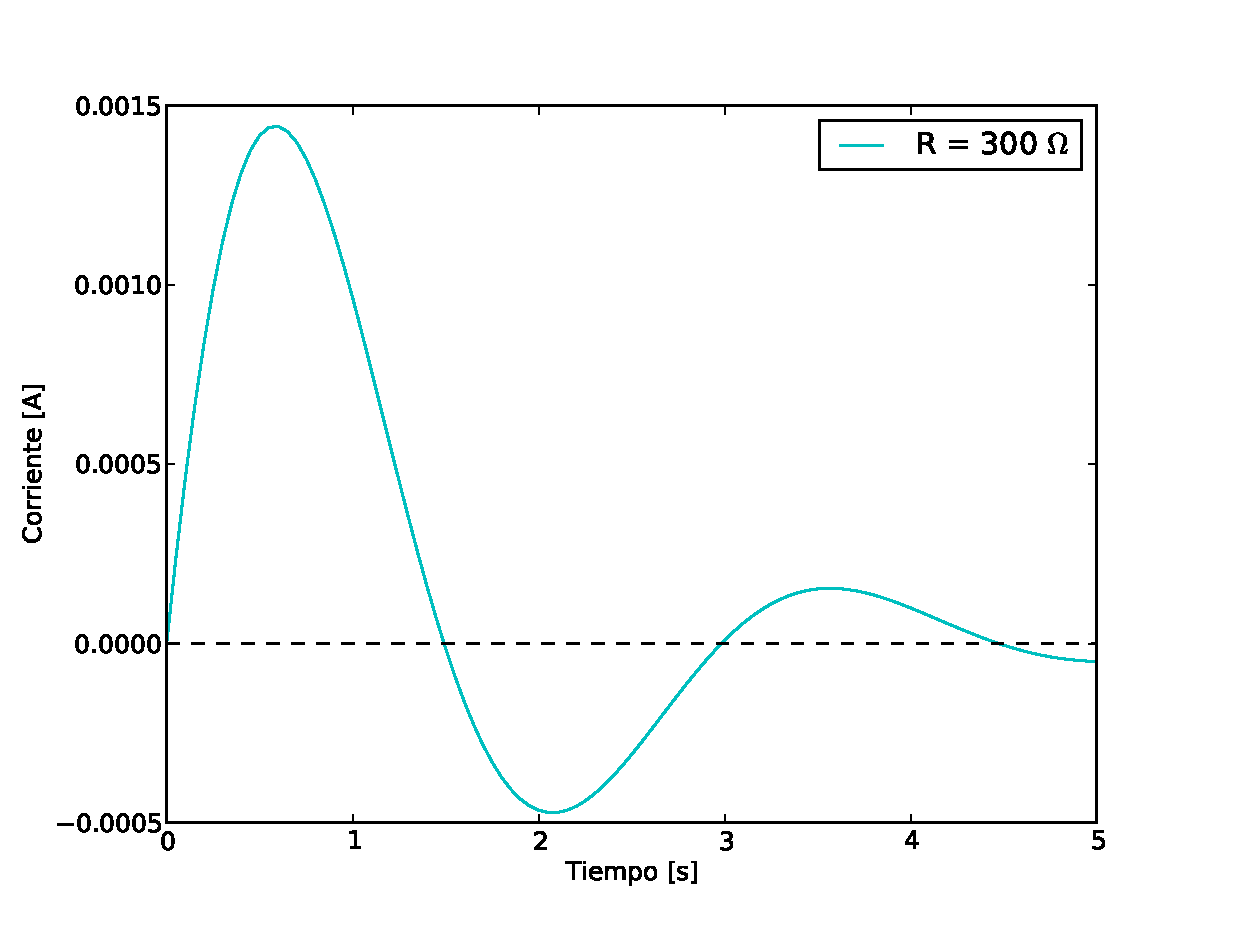
\includegraphics[scale=0.5]{SistemaElecRK4_04.eps} 
\end{figure}
\end{frame}
\begin{frame}
\frametitle{Soluci\'{o}n gr\'{a}fica con valores de $R$ superpuestos}
\begin{figure}
	\centering
	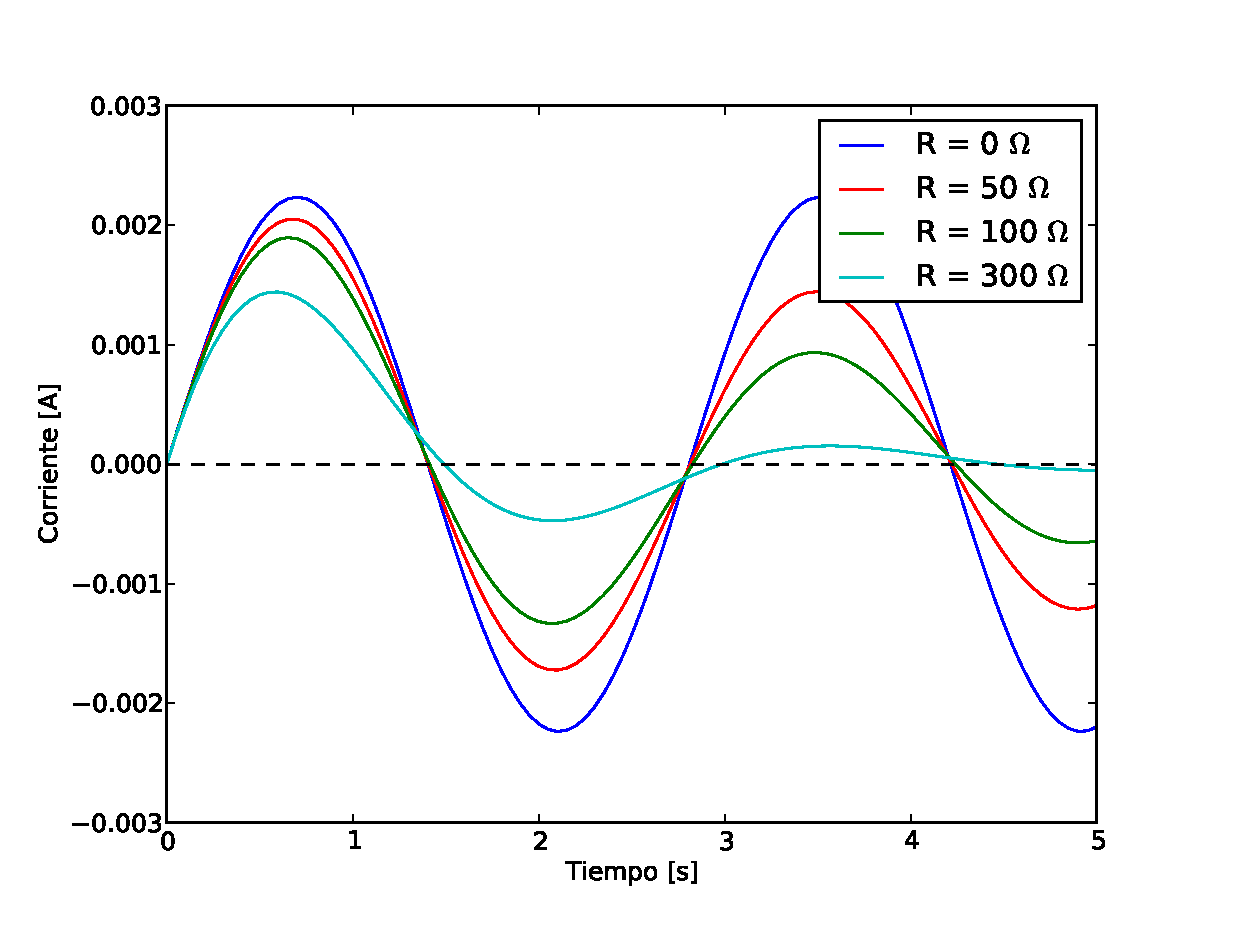
\includegraphics[scale=0.5]{SistemaElecRK4_05.eps} 
\end{figure}
\end{frame}
\begin{frame}[fragile]
\frametitle{Ejercicio a cuenta de examen}
En la figura se muestra un sistema de tres masas. Los desplazamientos de estas tres masas satisfacen las ecuaciones dadas por:
\fontsize{12}{12}\selectfont
\begin{eqnarray*} 
	M_{1} y''_{1} + B_{1} y'_{1} + K_{1} y_{1} - B_{1} y'_{2} - K_{2}y_{2} & = & F_{1}(t) \\
	-B_{1} y'_{1} - K_{1} y_{1} + M_{2} y''_{2} + B_{1} y'_{2} + (K_{1} + K_{2}) y_{2} - K_{2} y_{3} & = & 0 \\
	-K_{2} y_{2} + M_{3} y''_{3} + B_{2} y'_{3} + (K_{2} + K_{3}) y_{3} & = & F_{3}(t) 
\end{eqnarray*}
\begin{tikzpicture}[scale=0.65, font=\small]
	\tikzstyle{spring}=[thick,decorate,decoration={zigzag,pre length=0.1cm,post
  length=0.1cm,segment length=6}]
	\draw [->,thick] (-1,1.6) -- node [above, midway] {$F_{1}$}(0,1.6);
	\draw (0,-0.4) -- (0,0);
	\draw (-0.5,-0.1) -- (-0.5,-0.4);
	\draw [->](-0.5,-0.25) -- node [midway, below] {$y_{1}$}(0,-0.25);
	\draw (0,0) rectangle node {$M_{1}$}(2,2);
	\draw[spring] (2,1.7) -- node [above] {$k_{1}$} (4,1.7);
	\draw (2,0.5) -- (2.6,0.5);
	\draw (2.6,0.1) -- (2.6,0.9);
	\draw (2.6,0.1) -- (3,0.1);
	\draw (2.8,-0.3) node {$B_{1}$};
	\draw (2.6,0.9) -- (3.0,0.9);
	\draw (2.8,0.3) -- (2.8,0.7);
	\draw (2.8,0.5) -- (4,0.5);
	\draw (4,-0.4) -- (4,0);
	\draw (3.5,-0.1) -- (3.5,-0.4);
	\draw [->](3.5,-0.25) -- node [midway, below] {$y_{2}$}(4,-0.25);
	\draw (4,0) rectangle node {$M_{2}$}(6,2);
	\draw [spring] (6,1) -- node [below] {$k_{2}$} (8,1);
	\draw [->,thick] (7,1.6) -- node [above, midway] {$F_{3}$}(8,1.6);
	\draw (8,-0.4) -- (8,0);
	\draw (7.5,-0.1) -- (7.5,-0.4);
	\draw [->](7.5,-0.25) -- node [midway, below] {$y_{3}$}(8,-0.25);
	\draw (8,0) rectangle node {$M_{3}$} (10,2);
	\draw[spring] (10,1.7) -- node [above] {$k_{3}$} (12,1.7);
	\draw (10,0.5) -- (10.6,0.5);
	\draw (10.6,0.1) -- (10.6,0.9);
	\draw (10.6,0.1) -- (11,0.1);
	\draw (10.8,-0.3) node {$B_{2}$};
	\draw (10.6,0.9) -- (11.0,0.9);
	\draw (10.8,0.3) -- (10.8,0.7);
	\draw (10.8,0.5) -- (12,0.5);
	\draw [pattern=north east lines] (12,-0.5) rectangle (14,3);
\end{tikzpicture}
\end{frame}
\begin{frame}
Las constantes y condiciones iniciales son
\fontsize{12}{12}\selectfont
\begin{tabbing}
$K_{1} = K_{2} = K_{3} = 1$ \hspace{1.2cm} \= (constantes de los resortes, kgm/$s^{2}$) \\
$M_{1} = M_{2} = M_{3} = 1$ \> (masa, kg) \\
$F_{1}(t) = 1, F_{3}(t) = 0$ \> (fuerza, N) \\
$B_{1} = B_{2} =0.1$ \> (coeficientes de amortiguamiento, kg/s) \\
\\
$y_{1}(0) = y'_{1}(0) = y_{2}(0) = y'_{2}(0) = y_{3}(0) = y'_{3}(0) = 0$ \\
\> (condiciones iniciales)
\end{tabbing}
Resuelve y grafica las ecuaciones anteriores mediante RK4, para $0 \leq t \leq 30$ segundos y $h=0.1$ \\
\end{frame}
\begin{frame}
Hint: Definiendo
\[ y_{4} = y'_{1}, \hspace{1cm} y_{5} = y'_{2}, \hspace{1cm} y_{6} = y'_{3} \]
La ecuación inicial se escribe como un conjunto de seis EDO de primer orden, de la siguiente manera:
\begin{eqnarray*}
y'_{1} & = & y_{4} \\
y'_{2} & = & y_{5} \\
y'_{3} & = & y_{6} \\
y'_{4} & = & \left[ -B_{1} y_{4} - K_{1} y_{1} + B_{1} y_{5} + K_{2} y_{2} + F_{1} \right] / M_{1} \\
y'_{5} & = & \left[ B_{1} y_{4} + K_{1} y_{1} - B_{1} y_{5} - \left( K_{1} + K_{2} \right) y_{2} + K_{2} y_{3} \right] / M_{2}\\
y'_{6} & = & \left[ K_{2} y_{2} - B_{2} y_{6} - \left( K_{2} + K_{3} \right)y_{3} + F_{3} \right] / M_{3}
\end{eqnarray*}
\end{frame}
\begin{frame}[fragile]
\frametitle{Soluci\'{o}n al problema}
\begin{figure}
	\centering
	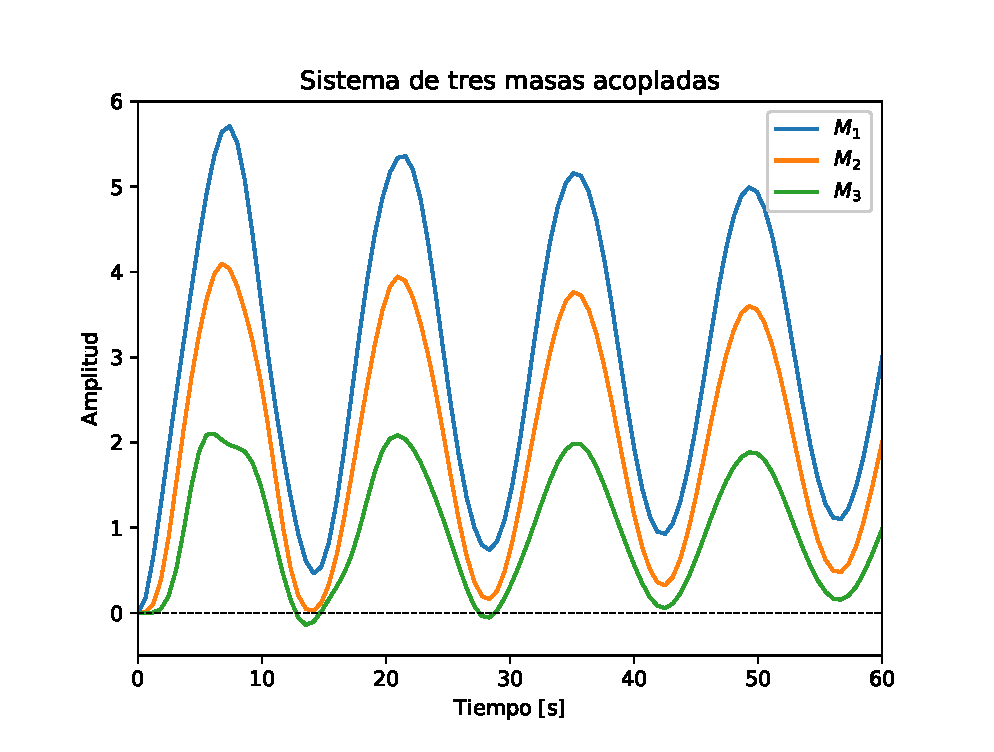
\includegraphics[scale=0.45]{SistemaTresMasasRK4.eps} 
\end{figure}
\end{frame}
\section{EDO con valores en las fronteras}
\begin{frame}
\frametitle{EDO con valores en las fronteras}
En los problemas de EDO unidimensionales con valores en la frontera, se pide que la soluci\'{o}n satisfaga las condiciones de frontera en ambos extremos del dominio unidimensional.
\\
\bigskip
La definici\'{o}n de las condiciones en la frontera, es parte fundamental de los problemas de este tipo.
\end{frame}
\begin{frame}
\frametitle{Problema de EDO con condiciones en la frontera}
Una varilla de 1 m de longitud colocada en el vac\'{i}o, se calienta mediante una corriente el\'{e}ctrica aplicada a la misma. La temperatura en los extremos se fija en $273$ K. 
\\
\bigskip
El calor se disipa de la superficie mediante la transferencia de calor por radiaci\'{o}n hacia al ambiente, cuya temperatura es de $273$ K. Con las siguiente constantes, determinar la distribuci\'{o}n de temperatura en dirección del eje.
\end{frame}
\begin{frame}
\begin{enumerate}
\item $ k= 60 W/mK$ conductividad t\'{e}rmica
\item $Q=50 W/m$ tasa de generaci\'{o}n de calor por \\ unidad de longitud de la barra
\item $\sigma = 5.67 \times 10^{-8} W/m^{2}K^{4}$ constante de Stefan-Boltzmann
\item $A=0.0001 m^{2}$ \'{a}rea de secci\'{o}n transversal
\item $P=0.01 m$ per\'{i}metro de la varilla
\end{enumerate}
La ecuaci\'{o}n de conducci\'{o}n de calor en la direcci\'{o}n del eje x es
\[ -Ak \dfrac{d^{2}}{dx^{2}} T + P \sigma (T^{4}-273^{4})=Q \hspace{1cm} 0<x<1.0 \]
con las condiciones en la frontera dadas por:
\[ T(0) = T(1.0) = 273 K \]
\end{frame}
\begin{frame}
Este problema es un problema condiciones en la frontera (espec\'{i}ficamente en $x=0$ y $x=1$), pero se puede resolver como un problema de condici\'{o}n inicial sobre la prueba de base y error. Definimos $y_{1}$ y $y_{2}$ como
\begin{eqnarray*}
y_{1} & = & T(x) \\
y_{2} & = & T'(x) 
\end{eqnarray*}
La ecuaci\'{o}n de conducci\'{o}n se puede re-escribir como un conjunto de dos EDO de primer orden como
\begin{eqnarray*}
y'_{1} & = & y_{2} \\
y'_{2} & = & \dfrac{P}{Ak} \sigma  \left( y^{4} - 273^{4} \right) - \dfrac{Q}{kA}
\end{eqnarray*}
\end{frame}
\end{document}